\documentclass[10pt,landscape,twocolumn]{article}

\RequirePackage{ifthen}
\RequirePackage{fancyhdr}
\RequirePackage{lastpage}
\RequirePackage{amssymb}
\RequirePackage{amsmath}
\RequirePackage{mathrsfs}
\RequirePackage{amsfonts}
\RequirePackage{color}
\RequirePackage[pdftex]{graphicx}
\RequirePackage{graphicx}

\usepackage{subfig}
\usepackage[margin=0.25in]{geometry}
\RequirePackage{amssymb}
\RequirePackage{amsmath}
\RequirePackage{mathrsfs}
\RequirePackage{amsfonts}
\newcommand{\pd}[2]{\frac{\partial #1}{\partial #2}}

\title{Test}

\begin{document}
% \maketitle


% \begin{table}[h]
% 	\centering
	\begin{tabular}{|l|c|c|}
		\hline
		Prefix & Abbreviation & Value \\
		\hline \hline
		Giga & $G$ & $10^9$ \\
		Mega & $M$ & $10^6$ \\
		Kilo & $k$ & $10^3$ \\
		\hline
		milli & $m$ & $10^{-3}$ \\
		micro & $\mu$ & $10^{-6}$ \\
		nano & $n$ & $10^{-9}$ \\
		pico & $p$ & $10^{-12}$ \\
		\hline
	\end{tabular}
% \end{table}


\begin{figure}[b]
	\centering
	\subfloat[1]{{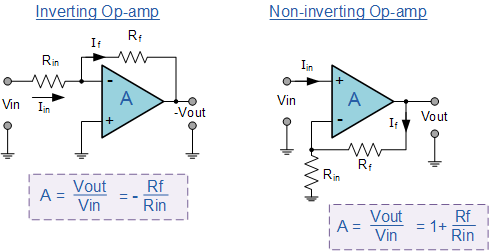
\includegraphics[width=0.33\textwidth]{invert-noninvert-opamp.png}}}
	% \qquad
	% \caption{Ohm's Law example circuit}
	\subfloat[2]{{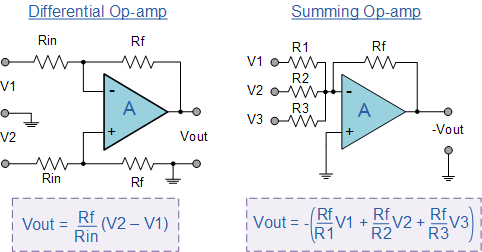
\includegraphics[width=0.33\textwidth]{diff-sum-opamp.png}}}
	% \caption{Ohm's Law example circuit}
	\subfloat[3]{{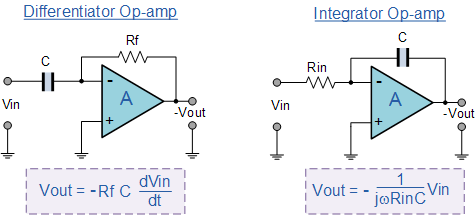
\includegraphics[width=0.33\textwidth]{diff-int-opamp.png}}}
	% \caption{Ohm's Law example circuit}
	% \label{fig: OhmsLawExampleSolution}
\end{figure}

% \begin{itemize}
% 	\item Node-voltage analysis: Nodes are particular points in a circuit. When many devices are connected to a particular point, you can make this node a reference node and think of it as having a voltage of 0 V. You then use it as a reference point to measure voltage for a particular node.
% With node-voltage analysis, you find unknown node voltages in a circuit using Kirchhoff’s current law. After finding the node voltages, you use current-voltage (i-v) relationships such as Ohm’s law to find device currents and use the node voltages to find device voltages.
% 	\item Mesh-current analysis: A mesh is a loop with no devices enclosed by the loop, where the mesh boundaries are those devices that form the loop.Mesh-current analysis lets you find unknown mesh currents in a circuit using Kirchhoff’s voltage law (KVL). Mesh equations are KVL equations with unknown mesh currents as variables. After finding mesh currents, you use i-v relationships to find device voltages.
% 	\item Superposition: For linear circuits with independent sources, you can use superposition to find the voltage and current output for a particular device. Superposition involves turning on sources one at a time while turning off the other sources. You turn off a current source by replacing it with an open circuit, and you turn off a voltage source by replacing it with a short circuit. To get the total output, you calculate the algebraic sum of individual contributions due to each source.
% 	\item Thévenin/Norton equivalents: Circuit analysis can become tedious when you’re trying different loads with the same source circuit. To save yourself some work, replace the source circuit with the Thévenin and Norton equivalents. Thévenin’s theorem says you can replace a linear network of sources and resistors between two terminals with one independent voltage source (VT) in series with one resistor (RT), and Norton’s theorem says you can replace the linear network of sources and resistors with one independent current source (IN) in parallel with one resistor (RN) — see the following figure. The equivalent circuits will hold for all loads (including open and short circuit loads) if they have the same voltage and current relationships across the terminals.
% Finding the Thévenin or Norton equivalent requires calculating the following variables: VT = VOC, IN = ISC, and RT = RN = VOC/ISC (where T stands for Thévenin, OC stands for an open-circuit load, N stands for Norton, and SCstands for a short circuit load). When you want to analyze different loads connected in series with the source circuit, the Thévenin equivalent is useful; when loads are connected in parallel with the source circuit, the Norton equivalent is a better choice. The two equivalents are related to each other by a source transformation.
%
% \end{itemize}

\begin{tabular}{|l|l|}
	\hline
	           & Forced Response Solution for $\tau = RC = \frac{L}{R}$\\
	\hline
	% Time Const & $\tau = RC = \frac{L}{R}$ \\
	Step       & $v_F(t)=Ke^{-\frac{t}{\tau}}$ \\
	Sinusoid   & $v_F(t)=a \cos(\omega t) + b \sin(\omega t)$ where $a=\frac{V_A}{1+\omega \tau}$ $b=\frac{\omega \tau V_A}{1+\omega \tau}$ \\
	Exp        & $v_F(t)=Ae^{-\alpha t}$ where $A=\frac{V_A}{1-\tau \alpha}$ \\
	\hline
\end{tabular}

\begin{tabular}{|l|c|l|l|}
	\hline
	        &   & Eqn & Units \\
	\hline
	Voltage & V & $v=\frac{dw}{dq}$ & $Volts = \frac{Joules}{Coulomb}$ \\
	Current & I & $i = \frac{dq}{dt}$ & $Amps = \frac{Coulomb}{seconds}$ \\
	Power   & P & $p = \frac{dw}{dt}=\frac{dw}{dq}\frac{dq}{dt}=v i$ & $Watts = \frac{Joules}{Seconds}$ \\
	\hline
\end{tabular}

\begin{tabular}{|l|c|c|}
	\hline
	         & Series & Parallel \\
	\hline
	Resistor  & $R_{eq} = \sum_{i=1}^n R_i$ & $\frac{1}{R_{eq}}=\sum_{i=1}^n \frac{1}{R_i}$ \\
	Capacitor & $\frac{1}{C_{eq}}=\sum_{i=1}^n \frac{1}{C_i}$ & $C_{eq} = \sum_{i=1}^n C_i$ \\
	Inductor  & $L_{eq} = \sum_{i=1}^n L_i$ & $\frac{1}{L_{eq}}=\sum_{i=1}^n \frac{1}{L_i}$ \\
	\hline
\end{tabular}

\begin{tabular}{|l|l|l|}
	\hline
	Part & Transient & Steady State \\
	\hline
	Capacitor  & short & open \\
	Inductor   & open & short \\
	\hline
\end{tabular}

\begin{tabular}{|l|l|l|}
	\hline
	Part & Transient & RX Circuit Solution \\
	\hline
	Capacitor & $i(t) = -C \pd{v}{t}$ & $v(t) = [ (V_o - V_A)e^{- \frac{t}{R_T C}}+V_A ] u(t)$ \\
	Inductor  & $v(t) = L \pd{i}{t}$  & $i(t) = [ (I_o - I_A)e^{- \frac{R_T t}{L}}+I_A ] u(t)$ \\
	\hline
\end{tabular}

\end{document}
